% Für Bindekorrektur als optionales Argument "BCORfaktormitmaßeinheit", dann
% sieht auch Option "twoside" vernünftig aus
% Näheres zu "scrartcl" bzw. "scrreprt" und "scrbook" siehe KOMA-Skript Doku
\documentclass[12pt,a4paper,titlepage,headinclude,bibtotoc]{scrartcl}


%---- Allgemeine Layout Einstellungen ------------------------------------------

% Für Kopf und Fußzeilen, siehe auch KOMA-Skript Doku
\usepackage[komastyle]{scrpage2}
\pagestyle{scrheadings}
\automark[section]{chapter}
\setheadsepline{0.5pt}[\color{black}]

%keine Einrückung
\parindent0pt

%Einstellungen für Figuren- und Tabellenbeschriftungen
\setkomafont{captionlabel}{\sffamily\bfseries}
\setcapindent{0em}

\usepackage{caption}

%---- Weitere Pakete -----------------------------------------------------------
% Die Pakete sind alle in der TeX Live Distribution enthalten. Wichtige Adressen
% www.ctan.org, www.dante.de

% Sprachunterstützung
\usepackage[ngerman]{babel}

% Benutzung von Umlauten direkt im Text
% entweder "latin1" oder "utf8"
\usepackage[utf8]{inputenc}

% Pakete mit Mathesymbolen und zur Beseitigung von Schwächen der Mathe-Umgebung
\usepackage{latexsym,exscale,amssymb,amsmath}

% Weitere Symbole
\usepackage[nointegrals]{wasysym}
\usepackage{eurosym}

% Anderes Literaturverzeichnisformat
%\usepackage[square,sort&compress]{natbib}

% Für Farbe
\usepackage{color}

% Zur Graphikausgabe
%Beipiel: \includegraphics[width=\textwidth]{grafik.png}
\usepackage{graphicx}

% Text umfließt Graphiken und Tabellen
% Beispiel:
% \begin{wrapfigure}[Zeilenanzahl]{"l" oder "r"}{breite}
%   \centering
%   \includegraphics[width=...]{grafik}
%   \caption{Beschriftung} 
%   \label{fig:grafik}
% \end{wrapfigure}
\usepackage{wrapfig}

% Mehrere Abbildungen nebeneinander
% Beispiel:
% \begin{figure}[htb]
%   \centering
%   \subfigure[Beschriftung 1\label{fig:label1}]
%   {\includegraphics[width=0.49\textwidth]{grafik1}}
%   \hfill
%   \subfigure[Beschriftung 2\label{fig:label2}]
%   {\includegraphics[width=0.49\textwidth]{grafik2}}
%   \caption{Beschriftung allgemein}
%   \label{fig:label-gesamt}
% \end{figure}
\usepackage{subfigure}
\usepackage{adjustbox}

% Caption neben Abbildung
% Beispiel:
% \sidecaptionvpos{figure}{"c" oder "t" oder "b"}
% \begin{SCfigure}[rel. Breite (normalerweise = 1)][hbt]
%   \centering
%   \includegraphics[width=0.5\textwidth]{grafik.png}
%   \caption{Beschreibung}
%   \label{fig:}
% \end{SCfigure}
\usepackage{sidecap}

% Befehl für "Entspricht"-Zeichen
\newcommand{\corresponds}{\ensuremath{\mathrel{\widehat{=}}}}

%Für chemische Formeln (von www.dante.de)
%% Anpassung an LaTeX(2e) von Bernd Raichle
\makeatletter
\DeclareRobustCommand{\chemical}[1]{%
  {\(\m@th
   \edef\resetfontdimens{\noexpand\)%
       \fontdimen16\textfont2=\the\fontdimen16\textfont2
       \fontdimen17\textfont2=\the\fontdimen17\textfont2\relax}%
   \fontdimen16\textfont2=2.7pt \fontdimen17\textfont2=2.7pt
   \mathrm{#1}%
   \resetfontdimens}}
\makeatother

%Si Einheiten
\usepackage{siunitx}

%c++ Code einbinden
\usepackage{listings}
\lstset{numbers=left, numberstyle=\tiny, numbersep=5pt}

%Differential
\newcommand{\dif}{\ensuremath{\mathrm{d}}}

%Boxen,etc.
\usepackage{fancybox}
\usepackage{empheq}

%Fußnoten auf gleiche Seite
\interfootnotelinepenalty=1000

%Dateien aus Unterverzeichnissen
\usepackage{import}

%Bibliography \bibliography{literatur} und \cite{gerthsen}
%\usepackage{cite}
\usepackage{babelbib}
\selectbiblanguage{ngerman}

\begin{document}

\begin{titlepage}
\centering
\textsc{\Large Anfängerpraktikum der Fakultät für
  Physik,\\[1.5ex] Universität Göttingen}

\vspace*{4.2cm}

\rule{\textwidth}{1pt}\\[0.5cm]
{\huge \bfseries
  Die spezifische\\[1.5ex]
  Wärme}\\[0.5cm]
\rule{\textwidth}{1pt}

\vspace*{3.0cm}

\begin{Large}
\begin{tabular}{ll}
Praktikant:
 	&  Felix Kurtz\\
 	&  Michael Lohmann\\

E-Mail: 
	&  felix.kurtz@stud.uni-goettingen.de\\
	& m.lohmann@stud.uni-goettingen.de\\

 Betreuer: & Phillip Bastian\\
 Versuchsdatum: &  13.03.2015\\
\end{tabular}
\end{Large}

\vspace*{0.8cm}

\begin{Large}
\fbox{
  \begin{minipage}[t][2.5cm][t]{6cm} 
    Testat:
  \end{minipage}
}
\end{Large}

\end{titlepage}

\tableofcontents

\newpage

\section{Einleitung}
\label{sec:einleitung}
Die spezifische Wärmespeicherkapazität ist eine wichtige Materialkonstante, da sie für viele alltäglichen Dinge essentiell ist.
Als Beispiel ist hier die Isolation zu nennen, die die Heizkosten moderat halten.
Hierfür ist es wichtig, Stoffe zu finden, die gut für diese Aufgabe geeignet sind.
Ein Versuch um Materialien zu charakterisieren wurde hier durchgeführt.

\section{Theorie}
\label{sec:theorie}

\section{Durchführung}
\label{sec:durchfuehrung}

\section{Auswertung}
\label{sec:auswertung}
\subsection{Temperaturverläufe}
\begin{align}
	T[\si{\celsius}]&=0.219+20.456 \cdot U - 0.302\cdot U^2+0.009\cdot U^3 \\
	\sigma_T&=20.456 - 0.604\cdot U+0.027\cdot U^2
\end{align}
\begin{figure}[!htb]
	\centering
	% GNUPLOT: LaTeX picture with Postscript
\begingroup
  \makeatletter
  \providecommand\color[2][]{%
    \GenericError{(gnuplot) \space\space\space\@spaces}{%
      Package color not loaded in conjunction with
      terminal option `colourtext'%
    }{See the gnuplot documentation for explanation.%
    }{Either use 'blacktext' in gnuplot or load the package
      color.sty in LaTeX.}%
    \renewcommand\color[2][]{}%
  }%
  \providecommand\includegraphics[2][]{%
    \GenericError{(gnuplot) \space\space\space\@spaces}{%
      Package graphicx or graphics not loaded%
    }{See the gnuplot documentation for explanation.%
    }{The gnuplot epslatex terminal needs graphicx.sty or graphics.sty.}%
    \renewcommand\includegraphics[2][]{}%
  }%
  \providecommand\rotatebox[2]{#2}%
  \@ifundefined{ifGPcolor}{%
    \newif\ifGPcolor
    \GPcolortrue
  }{}%
  \@ifundefined{ifGPblacktext}{%
    \newif\ifGPblacktext
    \GPblacktexttrue
  }{}%
  % define a \g@addto@macro without @ in the name:
  \let\gplgaddtomacro\g@addto@macro
  % define empty templates for all commands taking text:
  \gdef\gplbacktext{}%
  \gdef\gplfronttext{}%
  \makeatother
  \ifGPblacktext
    % no textcolor at all
    \def\colorrgb#1{}%
    \def\colorgray#1{}%
  \else
    % gray or color?
    \ifGPcolor
      \def\colorrgb#1{\color[rgb]{#1}}%
      \def\colorgray#1{\color[gray]{#1}}%
      \expandafter\def\csname LTw\endcsname{\color{white}}%
      \expandafter\def\csname LTb\endcsname{\color{black}}%
      \expandafter\def\csname LTa\endcsname{\color{black}}%
      \expandafter\def\csname LT0\endcsname{\color[rgb]{1,0,0}}%
      \expandafter\def\csname LT1\endcsname{\color[rgb]{0,1,0}}%
      \expandafter\def\csname LT2\endcsname{\color[rgb]{0,0,1}}%
      \expandafter\def\csname LT3\endcsname{\color[rgb]{1,0,1}}%
      \expandafter\def\csname LT4\endcsname{\color[rgb]{0,1,1}}%
      \expandafter\def\csname LT5\endcsname{\color[rgb]{1,1,0}}%
      \expandafter\def\csname LT6\endcsname{\color[rgb]{0,0,0}}%
      \expandafter\def\csname LT7\endcsname{\color[rgb]{1,0.3,0}}%
      \expandafter\def\csname LT8\endcsname{\color[rgb]{0.5,0.5,0.5}}%
    \else
      % gray
      \def\colorrgb#1{\color{black}}%
      \def\colorgray#1{\color[gray]{#1}}%
      \expandafter\def\csname LTw\endcsname{\color{white}}%
      \expandafter\def\csname LTb\endcsname{\color{black}}%
      \expandafter\def\csname LTa\endcsname{\color{black}}%
      \expandafter\def\csname LT0\endcsname{\color{black}}%
      \expandafter\def\csname LT1\endcsname{\color{black}}%
      \expandafter\def\csname LT2\endcsname{\color{black}}%
      \expandafter\def\csname LT3\endcsname{\color{black}}%
      \expandafter\def\csname LT4\endcsname{\color{black}}%
      \expandafter\def\csname LT5\endcsname{\color{black}}%
      \expandafter\def\csname LT6\endcsname{\color{black}}%
      \expandafter\def\csname LT7\endcsname{\color{black}}%
      \expandafter\def\csname LT8\endcsname{\color{black}}%
    \fi
  \fi
  \setlength{\unitlength}{0.0500bp}%
  \begin{picture}(7200.00,5040.00)%
    \gplgaddtomacro\gplbacktext{%
      \csname LTb\endcsname%
      \put(946,704){\makebox(0,0)[r]{\strut{} 290}}%
      \put(946,1286){\makebox(0,0)[r]{\strut{} 300}}%
      \put(946,1867){\makebox(0,0)[r]{\strut{} 310}}%
      \put(946,2449){\makebox(0,0)[r]{\strut{} 320}}%
      \put(946,3030){\makebox(0,0)[r]{\strut{} 330}}%
      \put(946,3612){\makebox(0,0)[r]{\strut{} 340}}%
      \put(946,4193){\makebox(0,0)[r]{\strut{} 350}}%
      \put(946,4775){\makebox(0,0)[r]{\strut{} 360}}%
      \put(1078,484){\makebox(0,0){\strut{} 0}}%
      \put(1794,484){\makebox(0,0){\strut{} 2}}%
      \put(2509,484){\makebox(0,0){\strut{} 4}}%
      \put(3225,484){\makebox(0,0){\strut{} 6}}%
      \put(3941,484){\makebox(0,0){\strut{} 8}}%
      \put(4656,484){\makebox(0,0){\strut{} 10}}%
      \put(5372,484){\makebox(0,0){\strut{} 12}}%
      \put(6087,484){\makebox(0,0){\strut{} 14}}%
      \put(6803,484){\makebox(0,0){\strut{} 16}}%
      \put(176,2739){\rotatebox{-270}{\makebox(0,0){\strut{}Temperatur $T$ [$\si\kelvin$]}}}%
      \put(3940,154){\makebox(0,0){\strut{}Zeit $t$ [min]}}%
    }%
    \gplgaddtomacro\gplfronttext{%
      \csname LTb\endcsname%
      \put(5816,4602){\makebox(0,0)[r]{\strut{}Aluminium}}%
      \csname LTb\endcsname%
      \put(5816,4382){\makebox(0,0)[r]{\strut{}Beryllium}}%
    }%
    \gplbacktext
    \put(0,0){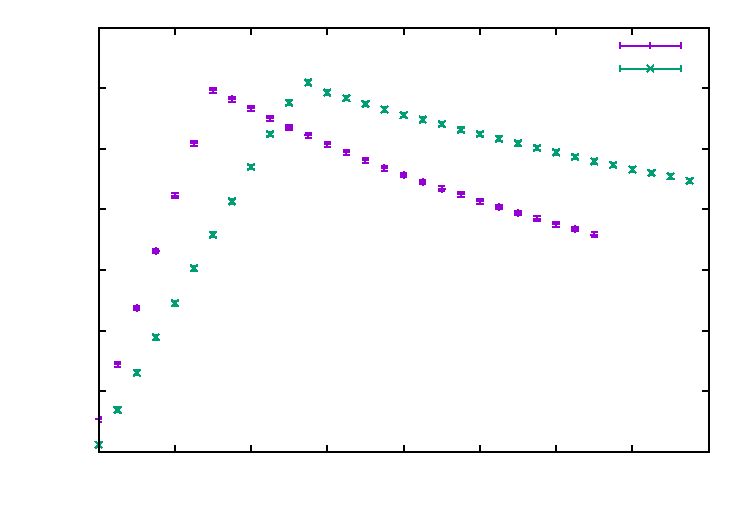
\includegraphics{Raumtemp}}%
    \gplfronttext
  \end{picture}%
\endgroup

	\caption{Raumtemperatur: Erhitzen und Abkühlen von Aluminium und Beryllium}
	\label{fig:Raumtemp}
\end{figure}

\begin{figure}[!htb]
	\centering
	% GNUPLOT: LaTeX picture with Postscript
\begingroup
  \makeatletter
  \providecommand\color[2][]{%
    \GenericError{(gnuplot) \space\space\space\@spaces}{%
      Package color not loaded in conjunction with
      terminal option `colourtext'%
    }{See the gnuplot documentation for explanation.%
    }{Either use 'blacktext' in gnuplot or load the package
      color.sty in LaTeX.}%
    \renewcommand\color[2][]{}%
  }%
  \providecommand\includegraphics[2][]{%
    \GenericError{(gnuplot) \space\space\space\@spaces}{%
      Package graphicx or graphics not loaded%
    }{See the gnuplot documentation for explanation.%
    }{The gnuplot epslatex terminal needs graphicx.sty or graphics.sty.}%
    \renewcommand\includegraphics[2][]{}%
  }%
  \providecommand\rotatebox[2]{#2}%
  \@ifundefined{ifGPcolor}{%
    \newif\ifGPcolor
    \GPcolortrue
  }{}%
  \@ifundefined{ifGPblacktext}{%
    \newif\ifGPblacktext
    \GPblacktexttrue
  }{}%
  % define a \g@addto@macro without @ in the name:
  \let\gplgaddtomacro\g@addto@macro
  % define empty templates for all commands taking text:
  \gdef\gplbacktext{}%
  \gdef\gplfronttext{}%
  \makeatother
  \ifGPblacktext
    % no textcolor at all
    \def\colorrgb#1{}%
    \def\colorgray#1{}%
  \else
    % gray or color?
    \ifGPcolor
      \def\colorrgb#1{\color[rgb]{#1}}%
      \def\colorgray#1{\color[gray]{#1}}%
      \expandafter\def\csname LTw\endcsname{\color{white}}%
      \expandafter\def\csname LTb\endcsname{\color{black}}%
      \expandafter\def\csname LTa\endcsname{\color{black}}%
      \expandafter\def\csname LT0\endcsname{\color[rgb]{1,0,0}}%
      \expandafter\def\csname LT1\endcsname{\color[rgb]{0,1,0}}%
      \expandafter\def\csname LT2\endcsname{\color[rgb]{0,0,1}}%
      \expandafter\def\csname LT3\endcsname{\color[rgb]{1,0,1}}%
      \expandafter\def\csname LT4\endcsname{\color[rgb]{0,1,1}}%
      \expandafter\def\csname LT5\endcsname{\color[rgb]{1,1,0}}%
      \expandafter\def\csname LT6\endcsname{\color[rgb]{0,0,0}}%
      \expandafter\def\csname LT7\endcsname{\color[rgb]{1,0.3,0}}%
      \expandafter\def\csname LT8\endcsname{\color[rgb]{0.5,0.5,0.5}}%
    \else
      % gray
      \def\colorrgb#1{\color{black}}%
      \def\colorgray#1{\color[gray]{#1}}%
      \expandafter\def\csname LTw\endcsname{\color{white}}%
      \expandafter\def\csname LTb\endcsname{\color{black}}%
      \expandafter\def\csname LTa\endcsname{\color{black}}%
      \expandafter\def\csname LT0\endcsname{\color{black}}%
      \expandafter\def\csname LT1\endcsname{\color{black}}%
      \expandafter\def\csname LT2\endcsname{\color{black}}%
      \expandafter\def\csname LT3\endcsname{\color{black}}%
      \expandafter\def\csname LT4\endcsname{\color{black}}%
      \expandafter\def\csname LT5\endcsname{\color{black}}%
      \expandafter\def\csname LT6\endcsname{\color{black}}%
      \expandafter\def\csname LT7\endcsname{\color{black}}%
      \expandafter\def\csname LT8\endcsname{\color{black}}%
    \fi
  \fi
    \setlength{\unitlength}{0.0500bp}%
    \ifx\gptboxheight\undefined%
      \newlength{\gptboxheight}%
      \newlength{\gptboxwidth}%
      \newsavebox{\gptboxtext}%
    \fi%
    \setlength{\fboxrule}{0.5pt}%
    \setlength{\fboxsep}{1pt}%
\begin{picture}(7200.00,5040.00)%
    \gplgaddtomacro\gplbacktext{%
      \csname LTb\endcsname%
      \put(946,704){\makebox(0,0)[r]{\strut{}$-180$}}%
      \put(946,1382){\makebox(0,0)[r]{\strut{}$-160$}}%
      \put(946,2061){\makebox(0,0)[r]{\strut{}$-140$}}%
      \put(946,2739){\makebox(0,0)[r]{\strut{}$-120$}}%
      \put(946,3418){\makebox(0,0)[r]{\strut{}$-100$}}%
      \put(946,4096){\makebox(0,0)[r]{\strut{}$-80$}}%
      \put(946,4775){\makebox(0,0)[r]{\strut{}$-60$}}%
      \put(1078,484){\makebox(0,0){\strut{}$0$}}%
      \put(2223,484){\makebox(0,0){\strut{}$5$}}%
      \put(3368,484){\makebox(0,0){\strut{}$10$}}%
      \put(4513,484){\makebox(0,0){\strut{}$15$}}%
      \put(5658,484){\makebox(0,0){\strut{}$20$}}%
      \put(6803,484){\makebox(0,0){\strut{}$25$}}%
    }%
    \gplgaddtomacro\gplfronttext{%
      \csname LTb\endcsname%
      \put(176,2739){\rotatebox{-270}{\makebox(0,0){\strut{}Temperatur $T$ [$^\circ C$]}}}%
      \put(3940,154){\makebox(0,0){\strut{}Zeit $t$ [min]}}%
      \csname LTb\endcsname%
      \put(5816,4602){\makebox(0,0)[r]{\strut{}Aluminium}}%
      \csname LTb\endcsname%
      \put(5816,4382){\makebox(0,0)[r]{\strut{}Beryllium}}%
    }%
    \gplbacktext
    \put(0,0){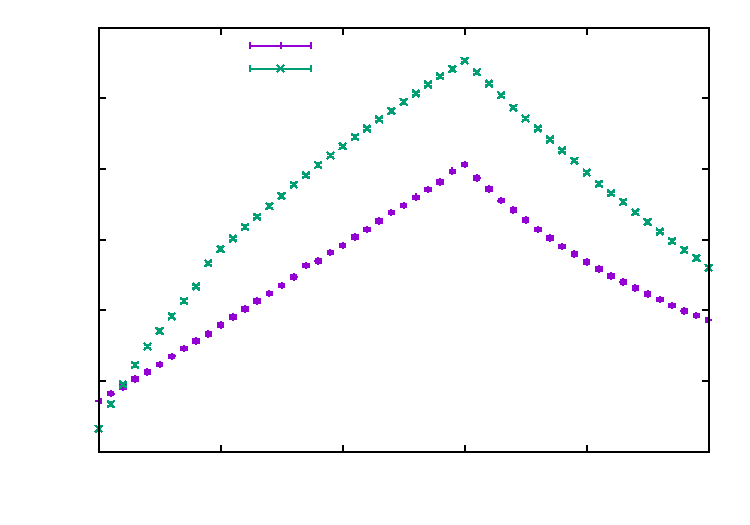
\includegraphics{Stickstofftemp}}%
    \gplfronttext
  \end{picture}%
\endgroup

	\caption{Stickstofftemperatur: Erhitzen und Abkühlen von Aluminium und Beryllium}
	\label{fig:Stickstofftemp}
\end{figure}

\subsection{Widerstand}
\begin{align}
	R&=\frac{U}{I}\\
	\sigma_R&=\frac{\sigma_U}{I}
\end{align}
\begin{figure}[!htb]
	\centering
	% GNUPLOT: LaTeX picture with Postscript
\begingroup
  \makeatletter
  \providecommand\color[2][]{%
    \GenericError{(gnuplot) \space\space\space\@spaces}{%
      Package color not loaded in conjunction with
      terminal option `colourtext'%
    }{See the gnuplot documentation for explanation.%
    }{Either use 'blacktext' in gnuplot or load the package
      color.sty in LaTeX.}%
    \renewcommand\color[2][]{}%
  }%
  \providecommand\includegraphics[2][]{%
    \GenericError{(gnuplot) \space\space\space\@spaces}{%
      Package graphicx or graphics not loaded%
    }{See the gnuplot documentation for explanation.%
    }{The gnuplot epslatex terminal needs graphicx.sty or graphics.sty.}%
    \renewcommand\includegraphics[2][]{}%
  }%
  \providecommand\rotatebox[2]{#2}%
  \@ifundefined{ifGPcolor}{%
    \newif\ifGPcolor
    \GPcolortrue
  }{}%
  \@ifundefined{ifGPblacktext}{%
    \newif\ifGPblacktext
    \GPblacktexttrue
  }{}%
  % define a \g@addto@macro without @ in the name:
  \let\gplgaddtomacro\g@addto@macro
  % define empty templates for all commands taking text:
  \gdef\gplbacktext{}%
  \gdef\gplfronttext{}%
  \makeatother
  \ifGPblacktext
    % no textcolor at all
    \def\colorrgb#1{}%
    \def\colorgray#1{}%
  \else
    % gray or color?
    \ifGPcolor
      \def\colorrgb#1{\color[rgb]{#1}}%
      \def\colorgray#1{\color[gray]{#1}}%
      \expandafter\def\csname LTw\endcsname{\color{white}}%
      \expandafter\def\csname LTb\endcsname{\color{black}}%
      \expandafter\def\csname LTa\endcsname{\color{black}}%
      \expandafter\def\csname LT0\endcsname{\color[rgb]{1,0,0}}%
      \expandafter\def\csname LT1\endcsname{\color[rgb]{0,1,0}}%
      \expandafter\def\csname LT2\endcsname{\color[rgb]{0,0,1}}%
      \expandafter\def\csname LT3\endcsname{\color[rgb]{1,0,1}}%
      \expandafter\def\csname LT4\endcsname{\color[rgb]{0,1,1}}%
      \expandafter\def\csname LT5\endcsname{\color[rgb]{1,1,0}}%
      \expandafter\def\csname LT6\endcsname{\color[rgb]{0,0,0}}%
      \expandafter\def\csname LT7\endcsname{\color[rgb]{1,0.3,0}}%
      \expandafter\def\csname LT8\endcsname{\color[rgb]{0.5,0.5,0.5}}%
    \else
      % gray
      \def\colorrgb#1{\color{black}}%
      \def\colorgray#1{\color[gray]{#1}}%
      \expandafter\def\csname LTw\endcsname{\color{white}}%
      \expandafter\def\csname LTb\endcsname{\color{black}}%
      \expandafter\def\csname LTa\endcsname{\color{black}}%
      \expandafter\def\csname LT0\endcsname{\color{black}}%
      \expandafter\def\csname LT1\endcsname{\color{black}}%
      \expandafter\def\csname LT2\endcsname{\color{black}}%
      \expandafter\def\csname LT3\endcsname{\color{black}}%
      \expandafter\def\csname LT4\endcsname{\color{black}}%
      \expandafter\def\csname LT5\endcsname{\color{black}}%
      \expandafter\def\csname LT6\endcsname{\color{black}}%
      \expandafter\def\csname LT7\endcsname{\color{black}}%
      \expandafter\def\csname LT8\endcsname{\color{black}}%
    \fi
  \fi
  \setlength{\unitlength}{0.0500bp}%
  \begin{picture}(7200.00,5040.00)%
    \gplgaddtomacro\gplbacktext{%
      \csname LTb\endcsname%
      \put(814,704){\makebox(0,0)[r]{\strut{} 60}}%
      \put(814,1383){\makebox(0,0)[r]{\strut{} 65}}%
      \put(814,2061){\makebox(0,0)[r]{\strut{} 70}}%
      \put(814,2740){\makebox(0,0)[r]{\strut{} 75}}%
      \put(814,3418){\makebox(0,0)[r]{\strut{} 80}}%
      \put(814,4097){\makebox(0,0)[r]{\strut{} 85}}%
      \put(814,4775){\makebox(0,0)[r]{\strut{} 90}}%
      \put(946,484){\makebox(0,0){\strut{} 290}}%
      \put(1922,484){\makebox(0,0){\strut{} 300}}%
      \put(2898,484){\makebox(0,0){\strut{} 310}}%
      \put(3875,484){\makebox(0,0){\strut{} 320}}%
      \put(4851,484){\makebox(0,0){\strut{} 330}}%
      \put(5827,484){\makebox(0,0){\strut{} 340}}%
      \put(6803,484){\makebox(0,0){\strut{} 350}}%
      \put(176,2739){\rotatebox{-270}{\makebox(0,0){\strut{}Widerstand $R$  [$\Omega$]}}}%
      \put(3874,154){\makebox(0,0){\strut{}Temperatur $T$ [$\si\kelvin$]}}%
    }%
    \gplgaddtomacro\gplfronttext{%
      \csname LTb\endcsname%
      \put(2266,4602){\makebox(0,0)[r]{\strut{}Aluminium}}%
      \csname LTb\endcsname%
      \put(2266,4382){\makebox(0,0)[r]{\strut{}Beryllium}}%
    }%
    \gplbacktext
    \put(0,0){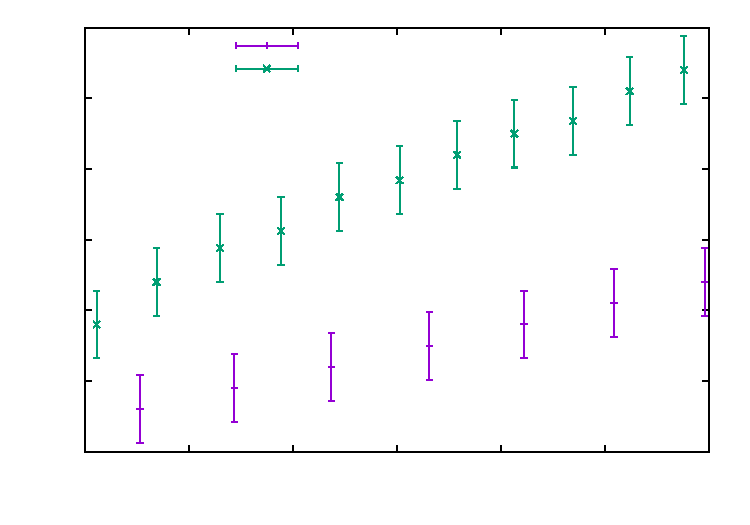
\includegraphics{Widerstand_Raum}}%
    \gplfronttext
  \end{picture}%
\endgroup

	\caption{Raumtemperatur: Widerstand des Cu-Drahtes}
	\label{fig:Widerstand_Raum}
\end{figure}

\begin{figure}[!htb]
	\centering
	% GNUPLOT: LaTeX picture with Postscript
\begingroup
  \makeatletter
  \providecommand\color[2][]{%
    \GenericError{(gnuplot) \space\space\space\@spaces}{%
      Package color not loaded in conjunction with
      terminal option `colourtext'%
    }{See the gnuplot documentation for explanation.%
    }{Either use 'blacktext' in gnuplot or load the package
      color.sty in LaTeX.}%
    \renewcommand\color[2][]{}%
  }%
  \providecommand\includegraphics[2][]{%
    \GenericError{(gnuplot) \space\space\space\@spaces}{%
      Package graphicx or graphics not loaded%
    }{See the gnuplot documentation for explanation.%
    }{The gnuplot epslatex terminal needs graphicx.sty or graphics.sty.}%
    \renewcommand\includegraphics[2][]{}%
  }%
  \providecommand\rotatebox[2]{#2}%
  \@ifundefined{ifGPcolor}{%
    \newif\ifGPcolor
    \GPcolortrue
  }{}%
  \@ifundefined{ifGPblacktext}{%
    \newif\ifGPblacktext
    \GPblacktexttrue
  }{}%
  % define a \g@addto@macro without @ in the name:
  \let\gplgaddtomacro\g@addto@macro
  % define empty templates for all commands taking text:
  \gdef\gplbacktext{}%
  \gdef\gplfronttext{}%
  \makeatother
  \ifGPblacktext
    % no textcolor at all
    \def\colorrgb#1{}%
    \def\colorgray#1{}%
  \else
    % gray or color?
    \ifGPcolor
      \def\colorrgb#1{\color[rgb]{#1}}%
      \def\colorgray#1{\color[gray]{#1}}%
      \expandafter\def\csname LTw\endcsname{\color{white}}%
      \expandafter\def\csname LTb\endcsname{\color{black}}%
      \expandafter\def\csname LTa\endcsname{\color{black}}%
      \expandafter\def\csname LT0\endcsname{\color[rgb]{1,0,0}}%
      \expandafter\def\csname LT1\endcsname{\color[rgb]{0,1,0}}%
      \expandafter\def\csname LT2\endcsname{\color[rgb]{0,0,1}}%
      \expandafter\def\csname LT3\endcsname{\color[rgb]{1,0,1}}%
      \expandafter\def\csname LT4\endcsname{\color[rgb]{0,1,1}}%
      \expandafter\def\csname LT5\endcsname{\color[rgb]{1,1,0}}%
      \expandafter\def\csname LT6\endcsname{\color[rgb]{0,0,0}}%
      \expandafter\def\csname LT7\endcsname{\color[rgb]{1,0.3,0}}%
      \expandafter\def\csname LT8\endcsname{\color[rgb]{0.5,0.5,0.5}}%
    \else
      % gray
      \def\colorrgb#1{\color{black}}%
      \def\colorgray#1{\color[gray]{#1}}%
      \expandafter\def\csname LTw\endcsname{\color{white}}%
      \expandafter\def\csname LTb\endcsname{\color{black}}%
      \expandafter\def\csname LTa\endcsname{\color{black}}%
      \expandafter\def\csname LT0\endcsname{\color{black}}%
      \expandafter\def\csname LT1\endcsname{\color{black}}%
      \expandafter\def\csname LT2\endcsname{\color{black}}%
      \expandafter\def\csname LT3\endcsname{\color{black}}%
      \expandafter\def\csname LT4\endcsname{\color{black}}%
      \expandafter\def\csname LT5\endcsname{\color{black}}%
      \expandafter\def\csname LT6\endcsname{\color{black}}%
      \expandafter\def\csname LT7\endcsname{\color{black}}%
      \expandafter\def\csname LT8\endcsname{\color{black}}%
    \fi
  \fi
    \setlength{\unitlength}{0.0500bp}%
    \ifx\gptboxheight\undefined%
      \newlength{\gptboxheight}%
      \newlength{\gptboxwidth}%
      \newsavebox{\gptboxtext}%
    \fi%
    \setlength{\fboxrule}{0.5pt}%
    \setlength{\fboxsep}{1pt}%
\begin{picture}(7200.00,5040.00)%
    \gplgaddtomacro\gplbacktext{%
      \csname LTb\endcsname%
      \put(682,704){\makebox(0,0)[r]{\strut{}$10$}}%
      \put(682,1213){\makebox(0,0)[r]{\strut{}$15$}}%
      \put(682,1722){\makebox(0,0)[r]{\strut{}$20$}}%
      \put(682,2231){\makebox(0,0)[r]{\strut{}$25$}}%
      \put(682,2740){\makebox(0,0)[r]{\strut{}$30$}}%
      \put(682,3248){\makebox(0,0)[r]{\strut{}$35$}}%
      \put(682,3757){\makebox(0,0)[r]{\strut{}$40$}}%
      \put(682,4266){\makebox(0,0)[r]{\strut{}$45$}}%
      \put(682,4775){\makebox(0,0)[r]{\strut{}$50$}}%
      \put(814,484){\makebox(0,0){\strut{}$100$}}%
      \put(1812,484){\makebox(0,0){\strut{}$120$}}%
      \put(2810,484){\makebox(0,0){\strut{}$140$}}%
      \put(3808,484){\makebox(0,0){\strut{}$160$}}%
      \put(4807,484){\makebox(0,0){\strut{}$180$}}%
      \put(5805,484){\makebox(0,0){\strut{}$200$}}%
      \put(6803,484){\makebox(0,0){\strut{}$220$}}%
    }%
    \gplgaddtomacro\gplfronttext{%
      \csname LTb\endcsname%
      \put(176,2739){\rotatebox{-270}{\makebox(0,0){\strut{}Widerstand $R$  [$\Omega$]}}}%
      \put(3808,154){\makebox(0,0){\strut{}Temperatur $T$ [$\si\kelvin]}}%
      \csname LTb\endcsname%
      \put(2134,4602){\makebox(0,0)[r]{\strut{}Aluminium}}%
      \csname LTb\endcsname%
      \put(2134,4382){\makebox(0,0)[r]{\strut{}Beryllium}}%
    }%
    \gplbacktext
    \put(0,0){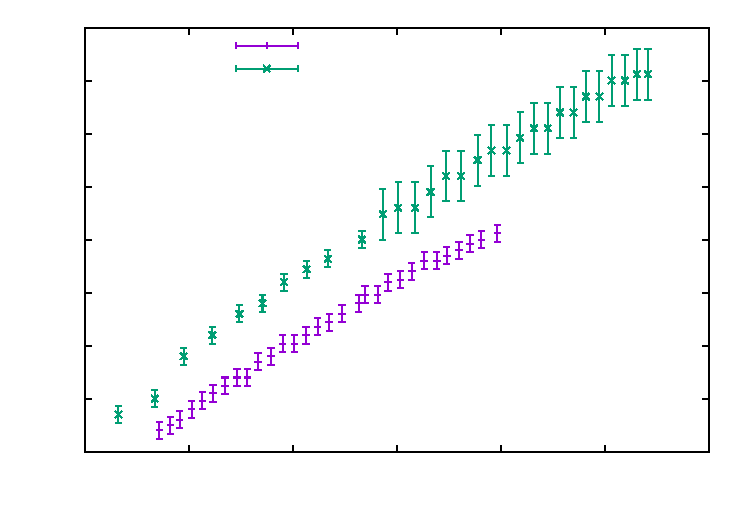
\includegraphics{Widerstand_Stick}}%
    \gplfronttext
  \end{picture}%
\endgroup

	\caption{Stickstofftemperatur: Widerstand des Cu-Drahtes}
	\label{fig:Widerstand_Stick}
\end{figure}

\subsection{Leistung}
\begin{align}
	P&=UI\\
	\sigma_P&=I\cdot\sigma_U
\end{align}
\begin{figure}[!htb]
	\centering
	% GNUPLOT: LaTeX picture with Postscript
\begingroup
  \makeatletter
  \providecommand\color[2][]{%
    \GenericError{(gnuplot) \space\space\space\@spaces}{%
      Package color not loaded in conjunction with
      terminal option `colourtext'%
    }{See the gnuplot documentation for explanation.%
    }{Either use 'blacktext' in gnuplot or load the package
      color.sty in LaTeX.}%
    \renewcommand\color[2][]{}%
  }%
  \providecommand\includegraphics[2][]{%
    \GenericError{(gnuplot) \space\space\space\@spaces}{%
      Package graphicx or graphics not loaded%
    }{See the gnuplot documentation for explanation.%
    }{The gnuplot epslatex terminal needs graphicx.sty or graphics.sty.}%
    \renewcommand\includegraphics[2][]{}%
  }%
  \providecommand\rotatebox[2]{#2}%
  \@ifundefined{ifGPcolor}{%
    \newif\ifGPcolor
    \GPcolortrue
  }{}%
  \@ifundefined{ifGPblacktext}{%
    \newif\ifGPblacktext
    \GPblacktexttrue
  }{}%
  % define a \g@addto@macro without @ in the name:
  \let\gplgaddtomacro\g@addto@macro
  % define empty templates for all commands taking text:
  \gdef\gplbacktext{}%
  \gdef\gplfronttext{}%
  \makeatother
  \ifGPblacktext
    % no textcolor at all
    \def\colorrgb#1{}%
    \def\colorgray#1{}%
  \else
    % gray or color?
    \ifGPcolor
      \def\colorrgb#1{\color[rgb]{#1}}%
      \def\colorgray#1{\color[gray]{#1}}%
      \expandafter\def\csname LTw\endcsname{\color{white}}%
      \expandafter\def\csname LTb\endcsname{\color{black}}%
      \expandafter\def\csname LTa\endcsname{\color{black}}%
      \expandafter\def\csname LT0\endcsname{\color[rgb]{1,0,0}}%
      \expandafter\def\csname LT1\endcsname{\color[rgb]{0,1,0}}%
      \expandafter\def\csname LT2\endcsname{\color[rgb]{0,0,1}}%
      \expandafter\def\csname LT3\endcsname{\color[rgb]{1,0,1}}%
      \expandafter\def\csname LT4\endcsname{\color[rgb]{0,1,1}}%
      \expandafter\def\csname LT5\endcsname{\color[rgb]{1,1,0}}%
      \expandafter\def\csname LT6\endcsname{\color[rgb]{0,0,0}}%
      \expandafter\def\csname LT7\endcsname{\color[rgb]{1,0.3,0}}%
      \expandafter\def\csname LT8\endcsname{\color[rgb]{0.5,0.5,0.5}}%
    \else
      % gray
      \def\colorrgb#1{\color{black}}%
      \def\colorgray#1{\color[gray]{#1}}%
      \expandafter\def\csname LTw\endcsname{\color{white}}%
      \expandafter\def\csname LTb\endcsname{\color{black}}%
      \expandafter\def\csname LTa\endcsname{\color{black}}%
      \expandafter\def\csname LT0\endcsname{\color{black}}%
      \expandafter\def\csname LT1\endcsname{\color{black}}%
      \expandafter\def\csname LT2\endcsname{\color{black}}%
      \expandafter\def\csname LT3\endcsname{\color{black}}%
      \expandafter\def\csname LT4\endcsname{\color{black}}%
      \expandafter\def\csname LT5\endcsname{\color{black}}%
      \expandafter\def\csname LT6\endcsname{\color{black}}%
      \expandafter\def\csname LT7\endcsname{\color{black}}%
      \expandafter\def\csname LT8\endcsname{\color{black}}%
    \fi
  \fi
    \setlength{\unitlength}{0.0500bp}%
    \ifx\gptboxheight\undefined%
      \newlength{\gptboxheight}%
      \newlength{\gptboxwidth}%
      \newsavebox{\gptboxtext}%
    \fi%
    \setlength{\fboxrule}{0.5pt}%
    \setlength{\fboxsep}{1pt}%
\begin{picture}(7200.00,5040.00)%
    \gplgaddtomacro\gplbacktext{%
      \csname LTb\endcsname%
      \put(682,704){\makebox(0,0)[r]{\strut{}$15$}}%
      \put(682,1213){\makebox(0,0)[r]{\strut{}$16$}}%
      \put(682,1722){\makebox(0,0)[r]{\strut{}$17$}}%
      \put(682,2231){\makebox(0,0)[r]{\strut{}$18$}}%
      \put(682,2740){\makebox(0,0)[r]{\strut{}$19$}}%
      \put(682,3248){\makebox(0,0)[r]{\strut{}$20$}}%
      \put(682,3757){\makebox(0,0)[r]{\strut{}$21$}}%
      \put(682,4266){\makebox(0,0)[r]{\strut{}$22$}}%
      \put(682,4775){\makebox(0,0)[r]{\strut{}$23$}}%
      \put(814,484){\makebox(0,0){\strut{}$290$}}%
      \put(1812,484){\makebox(0,0){\strut{}$300$}}%
      \put(2810,484){\makebox(0,0){\strut{}$310$}}%
      \put(3808,484){\makebox(0,0){\strut{}$320$}}%
      \put(4807,484){\makebox(0,0){\strut{}$330$}}%
      \put(5805,484){\makebox(0,0){\strut{}$340$}}%
      \put(6803,484){\makebox(0,0){\strut{}$350$}}%
    }%
    \gplgaddtomacro\gplfronttext{%
      \csname LTb\endcsname%
      \put(176,2739){\rotatebox{-270}{\makebox(0,0){\strut{}Leistung $P$  [W]}}}%
      \put(3808,154){\makebox(0,0){\strut{}Temperatur $T$ [$\si{\kelvin}$]}}%
      \csname LTb\endcsname%
      \put(2134,4602){\makebox(0,0)[r]{\strut{}Aluminium}}%
      \csname LTb\endcsname%
      \put(2134,4382){\makebox(0,0)[r]{\strut{}Beryllium}}%
    }%
    \gplbacktext
    \put(0,0){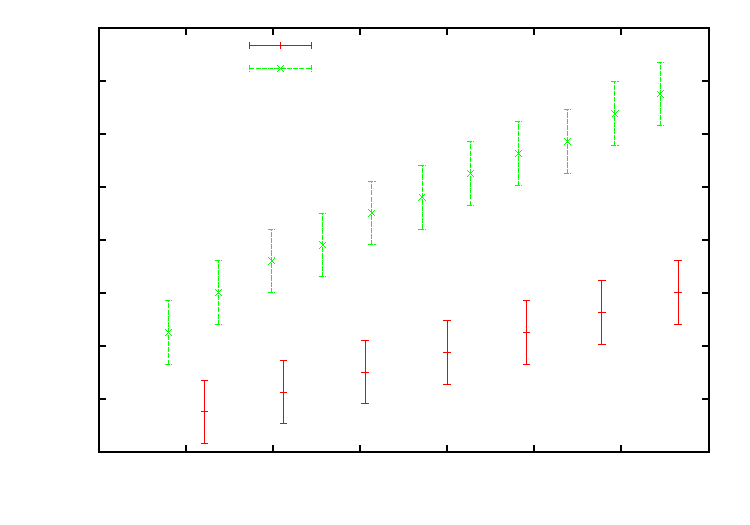
\includegraphics{Leistung_Raum}}%
    \gplfronttext
  \end{picture}%
\endgroup

	\caption{Raumtemperatur: beim Heizen hineingesteckte Leistung}
	\label{fig:Leistung_Raum}
\end{figure}

\begin{figure}[!htb]
	\centering
	% GNUPLOT: LaTeX picture with Postscript
\begingroup
  \makeatletter
  \providecommand\color[2][]{%
    \GenericError{(gnuplot) \space\space\space\@spaces}{%
      Package color not loaded in conjunction with
      terminal option `colourtext'%
    }{See the gnuplot documentation for explanation.%
    }{Either use 'blacktext' in gnuplot or load the package
      color.sty in LaTeX.}%
    \renewcommand\color[2][]{}%
  }%
  \providecommand\includegraphics[2][]{%
    \GenericError{(gnuplot) \space\space\space\@spaces}{%
      Package graphicx or graphics not loaded%
    }{See the gnuplot documentation for explanation.%
    }{The gnuplot epslatex terminal needs graphicx.sty or graphics.sty.}%
    \renewcommand\includegraphics[2][]{}%
  }%
  \providecommand\rotatebox[2]{#2}%
  \@ifundefined{ifGPcolor}{%
    \newif\ifGPcolor
    \GPcolortrue
  }{}%
  \@ifundefined{ifGPblacktext}{%
    \newif\ifGPblacktext
    \GPblacktexttrue
  }{}%
  % define a \g@addto@macro without @ in the name:
  \let\gplgaddtomacro\g@addto@macro
  % define empty templates for all commands taking text:
  \gdef\gplbacktext{}%
  \gdef\gplfronttext{}%
  \makeatother
  \ifGPblacktext
    % no textcolor at all
    \def\colorrgb#1{}%
    \def\colorgray#1{}%
  \else
    % gray or color?
    \ifGPcolor
      \def\colorrgb#1{\color[rgb]{#1}}%
      \def\colorgray#1{\color[gray]{#1}}%
      \expandafter\def\csname LTw\endcsname{\color{white}}%
      \expandafter\def\csname LTb\endcsname{\color{black}}%
      \expandafter\def\csname LTa\endcsname{\color{black}}%
      \expandafter\def\csname LT0\endcsname{\color[rgb]{1,0,0}}%
      \expandafter\def\csname LT1\endcsname{\color[rgb]{0,1,0}}%
      \expandafter\def\csname LT2\endcsname{\color[rgb]{0,0,1}}%
      \expandafter\def\csname LT3\endcsname{\color[rgb]{1,0,1}}%
      \expandafter\def\csname LT4\endcsname{\color[rgb]{0,1,1}}%
      \expandafter\def\csname LT5\endcsname{\color[rgb]{1,1,0}}%
      \expandafter\def\csname LT6\endcsname{\color[rgb]{0,0,0}}%
      \expandafter\def\csname LT7\endcsname{\color[rgb]{1,0.3,0}}%
      \expandafter\def\csname LT8\endcsname{\color[rgb]{0.5,0.5,0.5}}%
    \else
      % gray
      \def\colorrgb#1{\color{black}}%
      \def\colorgray#1{\color[gray]{#1}}%
      \expandafter\def\csname LTw\endcsname{\color{white}}%
      \expandafter\def\csname LTb\endcsname{\color{black}}%
      \expandafter\def\csname LTa\endcsname{\color{black}}%
      \expandafter\def\csname LT0\endcsname{\color{black}}%
      \expandafter\def\csname LT1\endcsname{\color{black}}%
      \expandafter\def\csname LT2\endcsname{\color{black}}%
      \expandafter\def\csname LT3\endcsname{\color{black}}%
      \expandafter\def\csname LT4\endcsname{\color{black}}%
      \expandafter\def\csname LT5\endcsname{\color{black}}%
      \expandafter\def\csname LT6\endcsname{\color{black}}%
      \expandafter\def\csname LT7\endcsname{\color{black}}%
      \expandafter\def\csname LT8\endcsname{\color{black}}%
    \fi
  \fi
  \setlength{\unitlength}{0.0500bp}%
  \begin{picture}(7200.00,5040.00)%
    \gplgaddtomacro\gplbacktext{%
      \csname LTb\endcsname%
      \put(814,704){\makebox(0,0)[r]{\strut{} 2}}%
      \put(814,1111){\makebox(0,0)[r]{\strut{} 3}}%
      \put(814,1518){\makebox(0,0)[r]{\strut{} 4}}%
      \put(814,1925){\makebox(0,0)[r]{\strut{} 5}}%
      \put(814,2332){\makebox(0,0)[r]{\strut{} 6}}%
      \put(814,2740){\makebox(0,0)[r]{\strut{} 7}}%
      \put(814,3147){\makebox(0,0)[r]{\strut{} 8}}%
      \put(814,3554){\makebox(0,0)[r]{\strut{} 9}}%
      \put(814,3961){\makebox(0,0)[r]{\strut{} 10}}%
      \put(814,4368){\makebox(0,0)[r]{\strut{} 11}}%
      \put(814,4775){\makebox(0,0)[r]{\strut{} 12}}%
      \put(946,484){\makebox(0,0){\strut{} 100}}%
      \put(1922,484){\makebox(0,0){\strut{} 120}}%
      \put(2898,484){\makebox(0,0){\strut{} 140}}%
      \put(3875,484){\makebox(0,0){\strut{} 160}}%
      \put(4851,484){\makebox(0,0){\strut{} 180}}%
      \put(5827,484){\makebox(0,0){\strut{} 200}}%
      \put(6803,484){\makebox(0,0){\strut{} 220}}%
      \put(176,2739){\rotatebox{-270}{\makebox(0,0){\strut{}Leistung $P$  [W]}}}%
      \put(3874,154){\makebox(0,0){\strut{}Temperatur $T$ [$\si\kelvin$]}}%
    }%
    \gplgaddtomacro\gplfronttext{%
      \csname LTb\endcsname%
      \put(2266,4602){\makebox(0,0)[r]{\strut{}Aluminium}}%
      \csname LTb\endcsname%
      \put(2266,4382){\makebox(0,0)[r]{\strut{}Beryllium}}%
    }%
    \gplbacktext
    \put(0,0){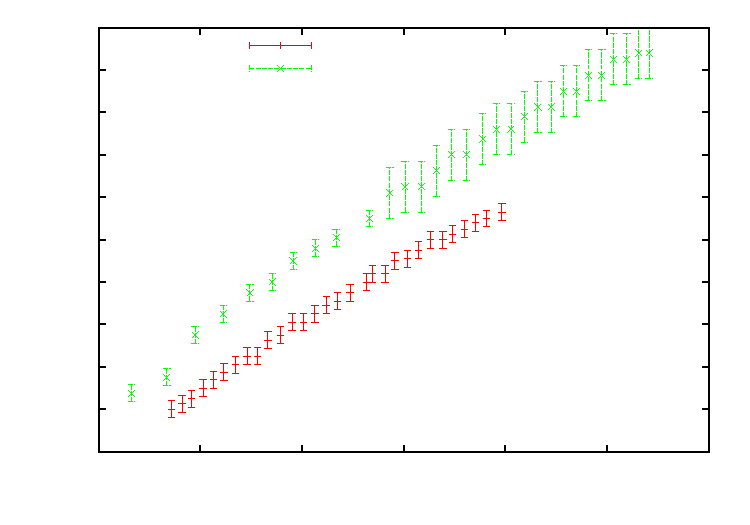
\includegraphics{Leistung_Stick}}%
    \gplfronttext
  \end{picture}%
\endgroup

	\caption{Stickstofftemperatur: beim Heizen hineingesteckte Leistung}
	\label{fig:Leistung_Stick}
\end{figure}

\subsection{molare Wärmekapazität}
\begin{align}
	C=\frac{P}{\frac{\dif T}{\dif t}|_\text{erw}+\frac{\dif T}{\dif t}|_\text{abk}}
\end{align}
Für das Erwärmen wird ein linearer Zusammenhang zwischen Temperatur und Zeit erwartet: $T(t)=a\cdot t +b$.
Dann ist $\frac{\dif T}{\dif t}|_\text{erw}=a$.
Für das Abkühlen kann man einen exponentiellen Abfall der Temperatur mit der Zeit annehmen: $T(t)=c\cdot e^{-\lambda t}$.
Somit ist $\frac{\dif T}{\dif t}|_\text{abk}=-\lambda\cdot T$.
\begin{align}
	c_m&=\frac{M}{m}\frac{P}{a+\lambda T}\\
	\sigma{c_m}&=\frac{M}{m}\sqrt{\frac{\sigma_P^2}{(a+\lambda T)^2}+\frac{P^2}{(a+\lambda T)^4}\cdot (\sigma_a^2+T^2 \sigma_\lambda^2+\lambda^2\sigma_T^2)}
\end{align}

\begin{table}[!htb]
	\centering
	\begin{tabular}{|c|c|c|}
		\hline
		& $a~[10^{-3}\cdot\si{\kelvin\per\second}}]$ & $\lambda~[10^{-5}\cdot\si{\per\second}}]$\\
		\hline
		Al RT	& $	303	\pm	2	$ & $	11.61	\pm	0.24	$ \\
		Be RT	& $	188.5	\pm	1.2	$ & $	7.61	\pm	0.14	$ \\
		Al Stickstoff	& $	74.85	\pm	0.23	$ & $	45.5	\pm	1.0	$ \\
		Be Stickstoff	& $	109	\pm	4	$ & $	60.48	\pm	0.18	$ \\
		\hline
	\end{tabular}
	\caption{Temperaturverläufe: gefittete Parameter}
	\label{tab:fitwerte}
\end{table}

\begin{figure}[!htb]
	\centering
	% GNUPLOT: LaTeX picture with Postscript
\begingroup
  \makeatletter
  \providecommand\color[2][]{%
    \GenericError{(gnuplot) \space\space\space\@spaces}{%
      Package color not loaded in conjunction with
      terminal option `colourtext'%
    }{See the gnuplot documentation for explanation.%
    }{Either use 'blacktext' in gnuplot or load the package
      color.sty in LaTeX.}%
    \renewcommand\color[2][]{}%
  }%
  \providecommand\includegraphics[2][]{%
    \GenericError{(gnuplot) \space\space\space\@spaces}{%
      Package graphicx or graphics not loaded%
    }{See the gnuplot documentation for explanation.%
    }{The gnuplot epslatex terminal needs graphicx.sty or graphics.sty.}%
    \renewcommand\includegraphics[2][]{}%
  }%
  \providecommand\rotatebox[2]{#2}%
  \@ifundefined{ifGPcolor}{%
    \newif\ifGPcolor
    \GPcolortrue
  }{}%
  \@ifundefined{ifGPblacktext}{%
    \newif\ifGPblacktext
    \GPblacktexttrue
  }{}%
  % define a \g@addto@macro without @ in the name:
  \let\gplgaddtomacro\g@addto@macro
  % define empty templates for all commands taking text:
  \gdef\gplbacktext{}%
  \gdef\gplfronttext{}%
  \makeatother
  \ifGPblacktext
    % no textcolor at all
    \def\colorrgb#1{}%
    \def\colorgray#1{}%
  \else
    % gray or color?
    \ifGPcolor
      \def\colorrgb#1{\color[rgb]{#1}}%
      \def\colorgray#1{\color[gray]{#1}}%
      \expandafter\def\csname LTw\endcsname{\color{white}}%
      \expandafter\def\csname LTb\endcsname{\color{black}}%
      \expandafter\def\csname LTa\endcsname{\color{black}}%
      \expandafter\def\csname LT0\endcsname{\color[rgb]{1,0,0}}%
      \expandafter\def\csname LT1\endcsname{\color[rgb]{0,1,0}}%
      \expandafter\def\csname LT2\endcsname{\color[rgb]{0,0,1}}%
      \expandafter\def\csname LT3\endcsname{\color[rgb]{1,0,1}}%
      \expandafter\def\csname LT4\endcsname{\color[rgb]{0,1,1}}%
      \expandafter\def\csname LT5\endcsname{\color[rgb]{1,1,0}}%
      \expandafter\def\csname LT6\endcsname{\color[rgb]{0,0,0}}%
      \expandafter\def\csname LT7\endcsname{\color[rgb]{1,0.3,0}}%
      \expandafter\def\csname LT8\endcsname{\color[rgb]{0.5,0.5,0.5}}%
    \else
      % gray
      \def\colorrgb#1{\color{black}}%
      \def\colorgray#1{\color[gray]{#1}}%
      \expandafter\def\csname LTw\endcsname{\color{white}}%
      \expandafter\def\csname LTb\endcsname{\color{black}}%
      \expandafter\def\csname LTa\endcsname{\color{black}}%
      \expandafter\def\csname LT0\endcsname{\color{black}}%
      \expandafter\def\csname LT1\endcsname{\color{black}}%
      \expandafter\def\csname LT2\endcsname{\color{black}}%
      \expandafter\def\csname LT3\endcsname{\color{black}}%
      \expandafter\def\csname LT4\endcsname{\color{black}}%
      \expandafter\def\csname LT5\endcsname{\color{black}}%
      \expandafter\def\csname LT6\endcsname{\color{black}}%
      \expandafter\def\csname LT7\endcsname{\color{black}}%
      \expandafter\def\csname LT8\endcsname{\color{black}}%
    \fi
  \fi
  \setlength{\unitlength}{0.0500bp}%
  \begin{picture}(7200.00,5040.00)%
    \gplgaddtomacro\gplbacktext{%
      \csname LTb\endcsname%
      \put(814,704){\makebox(0,0)[r]{\strut{} 0}}%
      \put(814,1383){\makebox(0,0)[r]{\strut{} 5}}%
      \put(814,2061){\makebox(0,0)[r]{\strut{} 10}}%
      \put(814,2740){\makebox(0,0)[r]{\strut{} 15}}%
      \put(814,3418){\makebox(0,0)[r]{\strut{} 20}}%
      \put(814,4097){\makebox(0,0)[r]{\strut{} 25}}%
      \put(814,4775){\makebox(0,0)[r]{\strut{} 30}}%
      \put(946,484){\makebox(0,0){\strut{} 100}}%
      \put(2117,484){\makebox(0,0){\strut{} 150}}%
      \put(3289,484){\makebox(0,0){\strut{} 200}}%
      \put(4460,484){\makebox(0,0){\strut{} 250}}%
      \put(5632,484){\makebox(0,0){\strut{} 300}}%
      \put(6803,484){\makebox(0,0){\strut{} 350}}%
      \put(176,2739){\rotatebox{-270}{\makebox(0,0){\strut{}molare Wärmekapatität $c_m$  [$\si[per-mode=fraction]{\joule\per\kelvin\per\mol}$]}}}%
      \put(3874,154){\makebox(0,0){\strut{}Temperatur $T$ [K]}}%
    }%
    \gplgaddtomacro\gplfronttext{%
      \csname LTb\endcsname%
      \put(5816,1537){\makebox(0,0)[r]{\strut{}Aluminium}}%
      \csname LTb\endcsname%
      \put(5816,1317){\makebox(0,0)[r]{\strut{}Beryllium}}%
      \csname LTb\endcsname%
      \put(5816,1097){\makebox(0,0)[r]{\strut{}Dulong-Petit-Wert}}%
      \csname LTb\endcsname%
      \put(5816,877){\makebox(0,0)[r]{\strut{}Be: Wert nach Debye}}%
    }%
    \gplbacktext
    \put(0,0){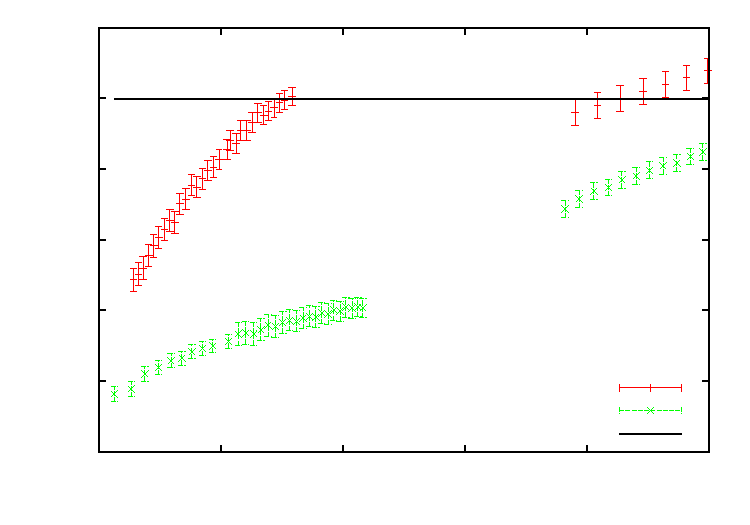
\includegraphics{waerme}}%
    \gplfronttext
  \end{picture}%
\endgroup

	\caption{molare Wärmekapazität bei verschiedenen Temperaturen für Aluminium und Beryllium sowie Vergleich mit dem Dulong-Petit-Wert}
	\label{fig:Leistung_Stick}
\end{figure}



\section{Diskussion}
\label{sec:diskussion}

\section{Anhang}

%\bibliography{literatur}
%\bibliographystyle{babalpha}

\end{document}
